% !TEX root= ../main.tex
\section{Inconsistencies in graph theories}
\label{sec:Inconsistencies in graph theories}
In this section, we will prove the existence of non-binary-derivable inconsistencies from graphs.
We will first prove a lemma, then apply this lemma to an extended version of the graph from Figure~\ref{fig:double_open_door} to show that its inconsistency is not binary-derivable.

Let $G$ be a digraph with a source vertex (a vertex with no predecessors) $x$.
Let $A$ and $B$ be two disjoint subgraphs of $G$ such that $N(A) \subseteq A$ and $N(B) \subseteq B$ and such that $N^-(A) \setminus A = N^-(B) \setminus B = \{ x\}$.
In words, nothing points out of $A$ and $B$ and only $x$ points in.
Note that $x$ might have additional successors.\par
\begin{figure}[!h]
  \centering
  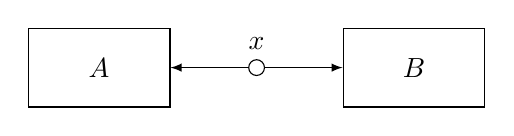
\begin{tikzpicture}
    [
    point/.style={circle,draw,inner sep=0pt,minimum size=2mm},
    collection/.style={rectangle,draw,inner sep=0pt,minimum height=10mm, minimum width= 18mm}
    ]
    \node (x) at (2,0) [point, label=above:$x$] {};
    \node (A) at (0,0) [collection] {$A$};
    \node (B) at (4,0) [collection] {$B$};
    \draw [-latex] (x) to (A);
    \draw [-latex] (x) to (B);
  \end{tikzpicture}
  \caption{Graph $G$}
  \label{fig:components_link}
\end{figure}
A couple of observations can be made from the above construction:
\begin{itemize}
  \item The vertex $x$ only appears in 1 OR-clause, since it is a source vertex.
  This is also the only OR-clause containing a vertex from both $A$ and $B$.
  We will call this OR-clause $X$ and formally define it as $N(x) \cup \{ x\}$.
  \item For any vertex $p$ in $A$ we have that $p$ only appears in axiomatic NAND-clauses together with either $t$ or other vertices in $A$.
  The same obviously holds for any vertex in $B$.
\end{itemize}
Based on graph $G$ from Figure~\ref{fig:components_link} we now introduce the following lemma:
\begin{lemma}
  Given two vertice $a \in A$ and $b \in B$; if $\ol{ab}$ is provable in Neg, then the proof must contain the OR-clause $X$.
\end{lemma}
The lemma will be proven by inducing over the length of the proof of $\ol{ab}$.
\begin{proof}
  In the base case, the proof length is 1, so $\ol{ab}$ is the direct conclusion from a premise with axioms only.
  \begin{figure}[!h]
    \centering
    \begin{prooftree*}
      \Hypo{\ol{ap}}
      \Hypo{\ol{bq}}
      \Hypo{\dots}
      \Infer[right label=$X$]3{\ol{ab}}
    \end{prooftree*}
    \caption{}
    \label{fig:ab_proof_bc}
  \end{figure}
  The premise must contain one axiom on the form $\ol{ap}$ and one on the form $\ol{bq}$.
  If either $p = x$ or $q = x$, then the OR-clause used in the proof step must be $X$, being the only OR-clause containing $x$.
  On the other hand, if neither $p$ nor $q$ equals $x$, then $p \in A$ and $q \in B$.
  Since $X$ is the only OR-clause containing vertices from both $A$ and $B$, $X$ is again our only choice.
  A proof of $\ol{ab}$ of length 1 must hence use the OR-clause $X$.

  For the inductive step, we assume that for any proof of length $k-1$; if it concludes with a NAND-clause $\ol{pq}$ such that $p$ and $q$ are from differen components, then it must use the OR-clause $X$ somewhere.
  This assumption makes us able to prove the inductive step in almost exactly the same way as with the base case.

  Suppose there is a proof of length $k$ concluding with $\ol{ab}$.
  Its immediate premise must contain one NAND-clause on the form $\ol{ap}$ and one on the form $\ol{bq}$.
  Again, if either $p=x$ or $q=x$, or if $p \in A$ and $q \in B$, the OR-clause $X$ must be used, by the same argument as in the base case.
  This leaves us with the case where either $p \nin A$ or $q \nin B$.
  Our induction hypothesis gives us that the proof of either of those contains $X$ somewhere.

  A proof of length $k$ concluding with $\ol{ab}$ must therefore use the OR-clause $X$, so we can conclude that \textit{any} proof of $\ol{ab}$ must contain $X$.
\end{proof}
  \begin{tikzpicture}
    [
    ]

